\documentclass{llncs}
\usepackage{graphicx}
\usepackage{caption}
\usepackage{subcaption}
\captionsetup{compatibility=false}
\usepackage{array}

\usepackage{amssymb}
\usepackage[numbers,sort]{natbib}
\usepackage{url}
\usepackage{multirow}
\renewcommand\bibname{References}
\newcommand{\keywords}[1]{\par\addvspace\baselineskip
\noindent\keywordname\enspace\ignorespaces#1}


%
\begin{document}

\title{A study on implementation and usage of web based programming assessment
system: Code}

\author{Tomche Delev\inst{1} \and Dejan Gjorgjevikj\inst{1}}

\institute{Faculty of Computer Science and Engineering
\email{\{tomche.delev,dejan.gjorgjevikj\}@finki.ukim.mk}}


\maketitle


\begin{abstract}
Implementing a web-based system for automatic assessment is a big step in the
introductionary programming courses. In this paper we study and report the
data generated by the usage of the system Code developed at the Faculty of
Computer Science and Engineering. The system supports compilation and execution
of programming problems in exercises and exams and it is used in many courses
that involve programming assignments. The analyzed data shows the differences in
working in laboratory settings, compared to practical exams. We also present the
results from plagiarism detection, and report significant cases of plagiarism in
introductionary courses. At the end we present the results from initial
qualitative evaluation of the system by surveying 48 students.

\keywords{Automatic assessment system, evaluation, plagiarism}
\end{abstract}

\section{Introduction}

In last three years, the trend of new enrolled students in CS is showing
constant increase. This trend directly effects the large number of students in
introductionary programming courses. The data at the Faculty of Computer Science
and Engineering (FCSE) shows that in 2012 and 2013 the number of enrolled
students in the introductionary programming course Structured Programming were 900 and
1029 respectively.

One step in better managing the learning process of large groups of students
was development and implementation of web based system for automatic assessment of programming
problems then called E-Lab \cite{delev2012lab} and now renamed to Code. The
initial idea of the system was to help tutors and instructors in identified
difficulties, that they have trying to assess all of the students' solutions.
Later on the system was also used in practical exams in courses that involve
programming assignments. The timed and informative feedback to students and
automatic assessment is top priority of the system.

Application of automatic assessment in programming assignments is suggested long
time ago \cite{hollingsworth1960automatic}. In the context of very large group
of students and the new MOOCs it may be the only solution to provide effective
feedback and grading. Speed, availability, consistency and objectivity of
assessment are some advantages mentioned in \cite{ala2005survey}, and
\cite{vujovsevic2013software} are showing that automatically generated grades
are highly correlated with instructor-assigned grades.

In this paper we present the experience and initial results from
implementing the system Code in two programming courses taught at FCSE. We
study the data generated by the usage of the system, and try to identify
patterns of usage that can reveal some potential new features or problems
with our system. We investigate the results from plagiarism detection and
present the results from qualitative evaluation on the system from
representative group of end users.

\section{Related Work}

The work on automatic assessment can be broadly categorized in research on
systems and tools and research on new methods and difficulties of novice
programmers. Examples of recent systems are eGrader \cite{shamsi2012intelligent}
graph-based grading system for Java introductionary programming courses,
CAT-SOOP \cite{hartz2012cat} a tool for automatic collection and assessment of
homework exercises and WeScheme \cite{yoo2011wescheme} that is a system
similar to Code \cite{delev2012lab} in using the web browser as coding
environment. In their work \cite{ihantola2010review} review most of the recent system.
They discuss the major features of these systems such the ways of defining tests
by teachers, resubmission policies, security issues and concluded that too many
systems are developed, mainly because most of the systems are closed and
collaboration is missing.

There are also studies on different approaches and learning methods that can be
helpful in designing, implementing or improvement of automatic assessment
systems. One such study is on the difficulties of novice programmers
\cite{lahtinen2005study}, where by surveying more than 500 students and
teachers, authors provide information of the difficulties experienced and
perceived when learning or teaching programming. One interesting conclusion they present is
that students overestimate their understanding, while the teachers think that
the course contents are more difficult for the students than the students
themselves. Students usually get the right perception lately during the exam
sessions.

Other interesting subject in research are studies on student programming bugs
and most occurred syntax errors. A one year empirical
study of student programming bugs is performed in \cite{bryce2010one}, where
authors conclude that approximately 22\% of the problems are due to problem solving
skills, while the remaining problems involve a combination of logic and syntax
problems. In the study on the most common syntax errors
\cite{denny2012all}, results are showing that many of these errors are
consuming large amount of student time, and even students with higher abilities
are not solving them more quickly. There are also studies that investigate
the dynamics and process of solving programming problems in novice programmers.
An analysis of patterns of debugging is presented in
\cite{ahmadzadeh2005analysis}, and in \cite{helminen2012students} the authors
try to reveal the process of solving programming problems that is mostly
invisible to the teachers. Using analysis of interaction traces they investigate
how students solve Parson's \cite{parsons2006parson} programming problems.

\section{Methodology and results}

In this paper we analyze the data generated from students using the
web-based system for automatic assessment of programming problems Code at the
Faculty of computer science and engineering in Skopje.
This system is in use from September 2012 and it is integral part in eight courses
that involve some kind of programming assignments in programming languages such
as C, C++ and Java. More than 2000 students are working on total 1296 problems,
organized in 367 problem sets, from which 165 (45\%) are exams. Students can
work on the system directly using the web-based code editor or they can use any
IDE, and then paste the code to run and test. By observing students in lab
and exam sessions, they mostly use the web-based editor in
introductionary programming courses or when making small changes in code, while
in more advanced courses they usually use IDEs such as Eclipse, NetBeans or
Code::Blocks.

\subsection{Data collected}

While students are using the system for solving the programming problems,
it is storing most of the data generated in the process. Among the
data collected by the system are the time when problem is
opened, and records for each student submission (attempt to solve the problem).
In order to test the correctness of their solution, students have two
options, to \emph{Run} or to \emph{Submit} the solution. When \emph{Run} is
performed the student code is saved and compiled, and if no syntax
errors are present, executed and tested using dynamic analysis on a sample test
case.
If errors are present in the compilation, the error and warning messages from the
compiler are returned as an output of the execution. If the compilation
succeed, the solution is executed, and the results from execution are shown next
to the expected sample output, so easy comparison on the outputs can be performed.
When saving the solution, if the content of the code is different from the
previous solution, it is stored as a new version of the solution, keeping the
old one. The system has implemented version history of the solutions, so
students can revert back to any previous version of their solution. This can be
very useful, specially to beginners who have not heard or tried any version
control system.
When users \emph{Submit} their solution, additionally to the steps performed
when running, the system saves a problem attempt record with time of the attempt
and result from testing the result on all the test cases of the given problem. The
result of the testing is the number of test cases passed, and if all test cases
passed, the attempt is marked as correct. Students can do unlimited
submissions and create as many problem attempts records. Even when the result from
submission is success, they still have the option to resubmit their solutions,
so as a result we can have multiple correct problem attempts by problem. In more
than two years of active usage of the system it has recorded more than 750,000
problem attempts and more than 1,000,000 versions of solutions.
A detailed study and analysis on part of this data is presented in this paper.

% \begin{figure}
% \centering
% 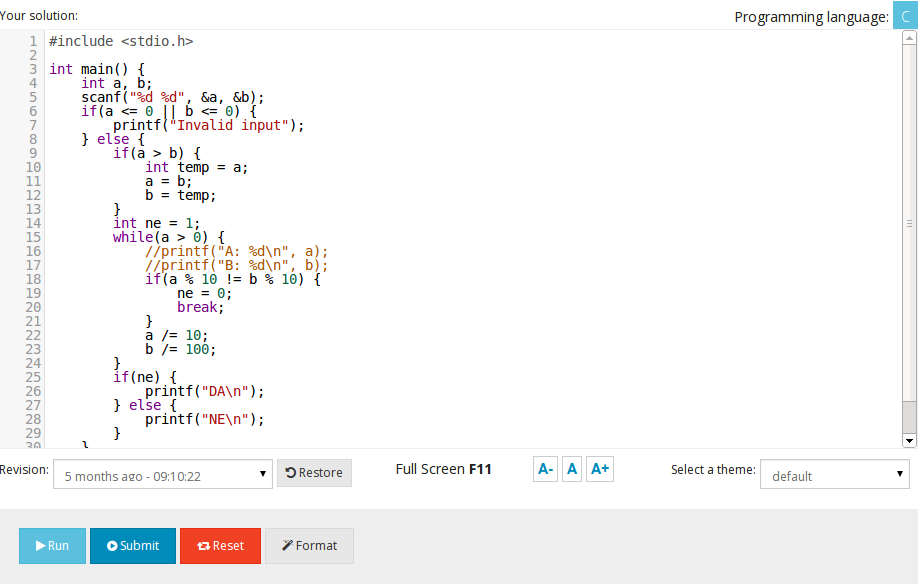
\includegraphics[width=.99\textwidth]{code_usage/editor}
% \caption{The web-based code editor in Code.}
% \label{fig:code_editor}
% \end{figure}

\subsection{The context}

From all the courses that are using the system, we report here on
data collected from the winter semester (September - December) 2012 of the following
two: Structured Programming (SP) and Advanced Programming (AP). Structured
Programming is a first year introductionary course thought in C, and Advanced
Programming is a second year more advanced elective course thought in Java.
1,029 students enrolled the course Structured Programming and each student had
to attend at least 80\% of 9 lab sessions, and had opportunity to take two midterm exams
and one final exam. Completing the lab sessions they could earn a total of 10\%
credit, and from solving the problems on the midterms or exam session they could
earn a total of 70\% credit towards their final grade in the course. The
students in this introductionary course are with different level of motivation
and there are significant number of students that are enrolling the courses
second time or third time. Advanced Programming was enrolled by 149 students,
and the settings of the course are similar to those in Structured Programming.
It should be noted that students in Advanced Programming were already familiar
with the system, by working on it in two previous courses from first year, and
they are more motivated because they chose the course by their own will.

We chose these courses because the system is in use second year, in both lab and
exam programming assignments.
\begin{figure}[htb]
\centering
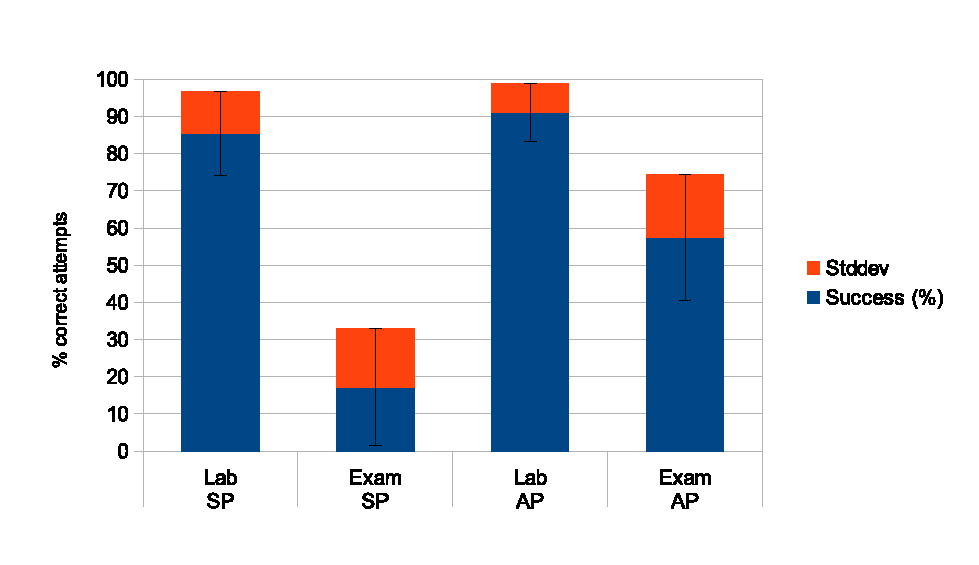
\includegraphics[width=.99\textwidth]{code_usage/problems_success_rate}
\caption{Problems success rate}
\label{fig:problems_success}
\end{figure}

\subsection{Problems success rate}

\begin{figure}[htb]
\centering
\begin{subfigure}{.5\textwidth}
  \centering
  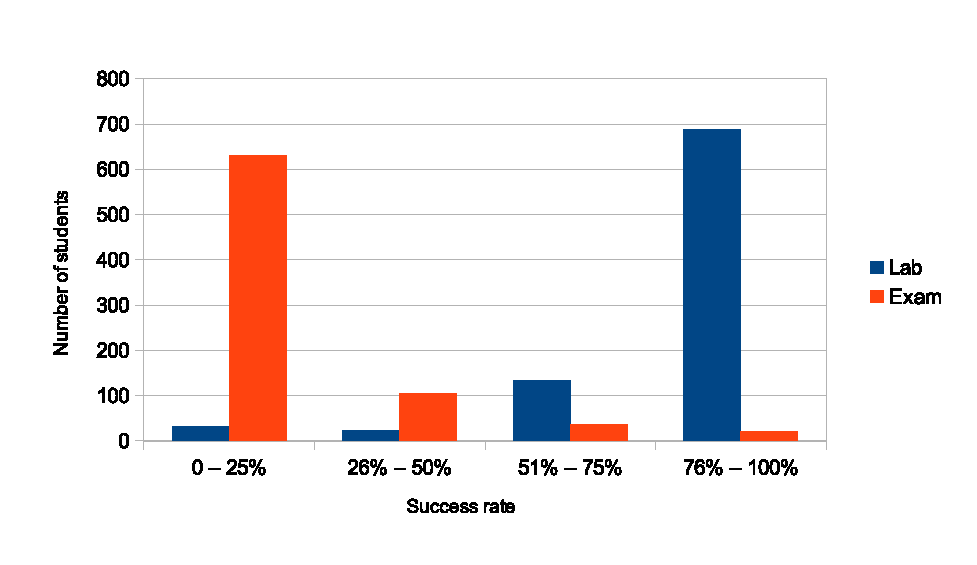
\includegraphics[width=\linewidth]{code_usage/sp_success_rate}
  \caption{SP success rate}
  \label{fig:sp_success_rate}
\end{subfigure}%
\begin{subfigure}{.5\textwidth}
  \centering
  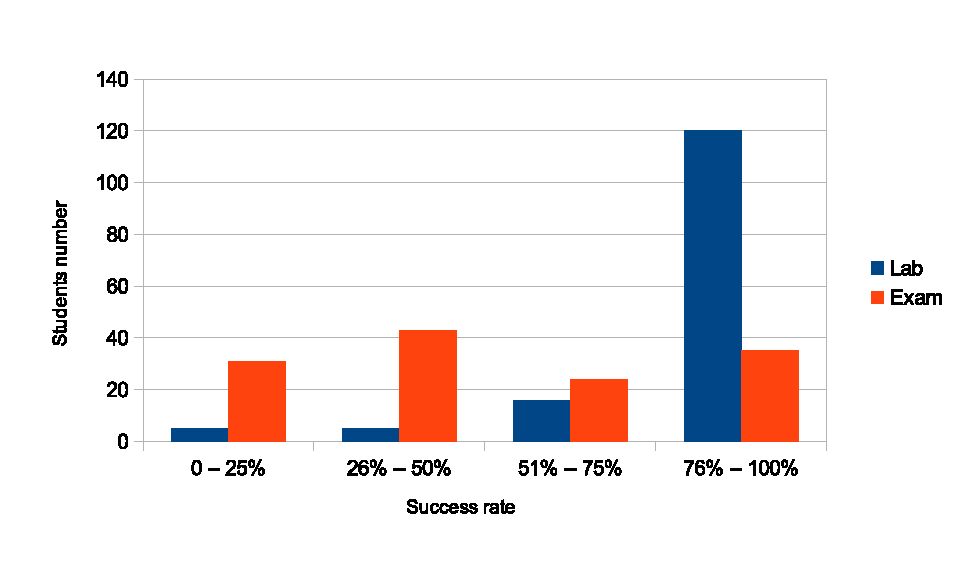
\includegraphics[width=\linewidth]{code_usage/ap_success_rate}
  \caption{AP success rate}
  \label{fig:ap_success_rate}
\end{subfigure}
\caption{Success rate on students}
\label{fig:students_success_rate}
\end{figure}
On figure \ref{fig:problems_success} the results
from success rate on problems in laboratory settings and exam settings
are presented and compared. We can note that success rate in lab
settings is higher then in exam settings, in both courses. Although the
problems difficulty in lab exercises is not lower then in exams, we can explain
this difference with the fact that lab problems are known to students, and they
are more prepared to solve them. Big impact on the success rate, especially in
the course SP, has the plagiarism in the solutions, reported later in the paper.
Figure \ref{fig:students_success_rate} presents the results on students
success rate.


\subsection{Source code evolution}

\newcolumntype{L}{>{\centering\arraybackslash}m{2cm}}

\begin{table}[htb]
\caption{Source code evolution data}
\begin{center}
\begin{tabular}{ |p{2.5cm}|l|L|L|L|L| }
\hline
 \textbf{Problem} & & \textbf{Average delta time (seconds)} & \textbf{Average
 compile success} & \textbf{Average deltas} & \textbf{Average lines} \\
\hline
\multirow{2}{*}{Recursion} 
& Correct & 408.7 & 0.77 & 1.72 & 29.8 \\
\cline{2-6}
& Incorrect & 172.4 & 0.49 & 1.47 & 25.0 \\
\hline
\multirow{2}{*}{Matrix}
& Correct & 137.6 & 0.90 & 1.85 & 40.4 \\
\cline{2-6}
& Incorrect & 228.1 & 0.61 & 1.79 & 32.6 \\
\hline
\multirow{2}{*}{Files}
 & Correct & 75.8 & 0.64 & 1.19 & 52.5 \\
 \cline{2-6}
 & Incorrect & 484.5 & 0.58 & 1.26 & 49.4 \\
\hline
\end{tabular}
\label{table:code_evolution}
\end{center}
\end{table}

On table \ref{table:code_evolution} the results from code evolution are
presented. We performed analysis on all solution versions for each student, from
the exam in January 2013. The solutions are divided in three groups by the type
of the problems, and the data is also split regarding the correctness of the
solution. We examined four metrics:

\begin{itemize}
  \item Average delta time - average time between attempts (seconds)
  \item Average compile success - average rate of compilation success
  \item Average deltas - average changes (deltas) between consecutive versions
  of source code
  \item Average lines - average lenght of the source code in number of lines.
\end{itemize}


On the first group of problems on the topic of recursion, where the
average length of the solutions is smallest, there is a big difference in the
average delta time between correct and incorrect solutions. This difference
tells us, that in solving more demanding problems in terms of thinking the
algorithm for the solution, the students who solve correctly spend more time
thinking the next change in the code. As opposed to them, students who did not
solve the problem correctly, worked with trial and error method, and did not
succeeded. The average deltas between new versions of solutions in all problems,
means that students mostly make from one to two changes in code between
attempts.
The average compilation success indicates that students who solved the problems are
also better in writing syntax correct code.

\section{Reports on plagiarism}

Plagiarism in source code in programming assignments is a serious issue in most
undergraduate courses that involve programming. In a study in 2004 at School of
Computing at the National University of Singapore, 181 students admitted
plagiarism \cite{tsang2005survey}, and the Centre for Academic Integrity (CAI)
reported that 40\% of 50,000 students at more than 60 universities admitted
plagiarism \cite{jocoy2006plagiarism}. Students involved in plagiarism learn a
lot less than their honest colleagues, they harm the reputation of their own
institutions, and reduce value of their own degrees.

\begin{table}[htb]
\caption{Results on plagiarism detection using MOSS}
\begin{center}
\begin{tabular}{ |l|L|L|L|L| }
\hline
Course & Settings & Average percentage match & Average lines matched & Potential
plagiarism pairs
\\
\hline 
\multirow{2}{*}{SP} & Lab & 52.04\% & 16.37 & 3869 \\
 & Exam & 22.74\% & 8.06 & 20 \\
\hline
\multirow{2}{*}{AP} & Lab & 10.08\% & 28.22 & 1 \\
 & Exam  & 10.26\% & 20.12 & 2 \\
\hline
\end{tabular}
\label{table:plagiarism_results}
\end{center}
\end{table}

\begin{figure}[htb]
\centering
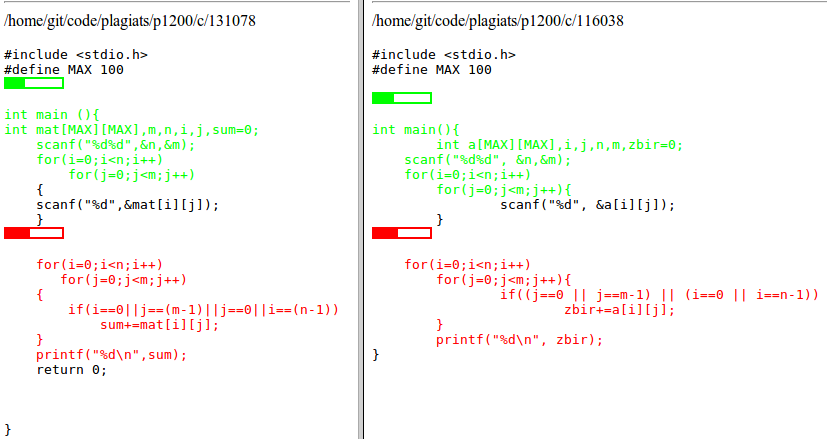
\includegraphics[width=.99\textwidth]{code_usage/plagiat_example}
\caption{Plagiarism example}
\label{fig:plagiats_example}
\end{figure}

Having in mind the importance of plagiarism detection, in our system we have
integrated one of the most efficient systems for that purpose, MOSS (Measure of
software similarity) \cite{aiken1994measure}. Before starting the winter
semester in 2013 the students were clearly informed that their solutions in the
system will be checked for plagiarism, and subsequently the involved parties will be
sanctioned. The results presented on table \ref{table:plagiarism_results} are
showing evidence of plagiarism mostly in laboratory settings in SP course, where
students have the freedom to share or use copied solutions. By examining
details of plagiarism cases, we discovered that in plagiarism were involved the
high achievers and low achievers, since latter mostly copied
solutions from the former. When directly presented the evidence, most of the
students admitted the plagiarism and regretted the action.

On figure \ref{fig:plagiats_example} we show example of the results from MOSS
system, where plagiarism is detected. Lines matched are colored green and red
and in this case it is a clear indicator that these two solutions
are strong case of plagiarism.

While in all academic settings it is still very import to address plagiarism in
every form, in a new learning model offered by MOOCs, where learning is no
longer for credits and grades, most of the factors contributing to plagiarism
may be eliminated. This is an important difference between MOOCs and traditional
courses. In the latter, the need for plagiarism detection and action against
plagiarism is paramount while in MOOCs it may serve no purpose.

\section{Evaluation}

\begin{table}[htb]
\caption{General usage questions}
\begin{center}
\begin{tabular}{ |p{5cm}|p{5cm}|l| }
\hline
\multirow{5}{*}{I used Code in?} & 1. Structured Programming (C) & 40\% \\
\cline{2-3}
 & 2. Object Oriented Programming (C++/Java) & 49\% \\
 \cline{2-3}
 & 3. Algorithms and Data Structures (C/Java) & 5\% \\
 \cline{2-3}
 & 4. Advanced Programming (Java) & 3\% \\
 \cline{2-3}
 & 5. Advanced Algorithms (Java) & 3\% \\
 \cline{2-3}
\hline
\multirow{2}{*}{I access Code from?} & 1. Faculty labs & 38\% \\
 & 2. From anywhere & 62\% \\
 \hline
\multirow{2}{5cm}{Do you want access from anywhere?} & Yes & 98\% \\
\cline{2-3}
 & No & 2\% \\
\hline
\multirow{4}{*}{How often do you use Code?} & 1. I don't use it & 1\% \\
\cline{2-3}
 & 2. Once a week & 42\% \\
 \cline{2-3}
 & 3. 2-3 times a week & 42\% \\
 \cline{2-3}
 & 4. More than 3 times a week & 15\% \\
 \cline{2-3}
\hline
\end{tabular}
\label{table:general_questions}
\end{center}
\end{table}
In the following tables we present the results from the initial evaluation of
the system by conducting a survey on group of 48 students in period of 10 days
at the end of summer semester in 2013. The questions were organized in
three groups. The first group of questions presented in table
\ref{table:general_questions} are general question about the usage of the
system. The first question shows that most of the responders (89\%) are from the
introductionary courses. The rest of responds are showing that users access
code at least once per week, not only from the faculty labs and strongly prefer
the access to be allowed from anywhere.
\begin{table}[htb]
\caption{System evaluation questions (1-5 grades)}
\begin{center}
\begin{tabular}{ |p{5cm}|l|l|l|l|l| }
\hline
Simple to use? & 1 (0\%) & 2 (2\%) & 3 (10\%) & 4 (21\%) & 5 (67\%) \\
\hline
Quality of presentation in problem view? & 1 (0\%) & 2 (13\%) & 3 (6\%) & 4
(21\%) & 5 (60\%)
\\
\hline
Code editor functionality? & 1 (4\%) & 2 (13\%) & 3 (13\%) & 4 (40\%) & 5 (31\%)
\\
\hline
Performance and speed? & 1 (0\%) & 2 (6\%) & 3 (6\%) & 4 (31\%) & 5 (56\%) \\
\hline
Do you think Code helps you in correctly solving the problem? &
\multicolumn{3}{l|}{Yes (62\%)} & \multicolumn{2}{l|}{No (38\%)}
 \\
\hline
When using Code? & \multicolumn{2}{p{2.5cm}|}{First use IDE and then copy the
solution (83\%)} & \multicolumn{2}{p{2.5cm}|}{Use the web-based code editor
(13\%)} & Other (4\%) \\
\hline
\end{tabular}
\label{table:system_evaluation}
\end{center}
\end{table}

On table \ref{table:system_evaluation} the presented results from the survey are
showing that students are generally satisfied with the simplicity of usage of
the system, they strongly rate the functionality and the performance of the system,
and most of them think that Code helps them in correctly solving the problem.
Also the majority of students (83\%) first use IDE and then copy the solution to
test and get feedback information.
\begin{table}[htb]
\caption{Learning programming}
\begin{center}
\begin{tabular}{ |p{4cm}|p{7cm}|l| }
\hline
\multirow{3}{4cm}{Where do you feel that you most learn (programming)?} &
1. Lectures & 4\%\\
\cline{2-3}
 & 2. TA Exams lectures & 17\% \\
 \cline{2-3}
 & 3. Lab exercises & 31\% \\
 \cline{2-3}
 & 4. Individual learning & 31\% \\
 \cline{2-3}
 & 5. Solving problems in Code & 5\% \\
 \cline{2-3}
 & 6. Other & 6\%\\
\hline
\multirow{3}{4cm}{What kind of materials helps you most in learning?} &
1. Books on subject & 13\%\\
\cline{2-3}
 & 2. Lectures slides & 15\% \\
\cline{2-3}
 & 3. Exercises questions and answers & 4\% \\
\cline{2-3} 
 & 4. Example problems with solutions & 46\% \\
 \cline{2-3}
 & 5. Interactive visualization of solutions & 13\% \\
 \cline{2-3}
 & 6. Other & 10\%\\
\hline
\multirow{3}{4cm}{While solving problem on code I mostly need help in?} &
1. Understand a problem and think of algorithm & 21\%\\
\cline{2-3}
 & 2. Implementing (coding) my solution & 27\% \\
 \cline{2-3}
 & 3. Locating and fixing errors in my solution & 46\% \\
 \cline{2-3}
 & 4. Other & 6\%\\
\hline
\multirow{3}{4cm}{What kind of help would be useful to be implemented?} &
1. Automatically showing relevant materials with similar problems and solutions
& 63\%\\
\cline{2-3}
 & 2. Direct communication with tutors over chat & 23\% \\
 \cline{2-3}
 & 3. Other & 7\%\\
\hline
\end{tabular}
\label{table:learning_programming}
\end{center}
\end{table}

From the results of the third group of questions presented in table
\ref{table:learning_programming} students feel that they learn most in lab
exercises and by doing individual work, from learning materials they prefer
example problems with solutions. On questions about further improvement,
the students expressed the need of help on locating and fixing errors in their
solutions. Also, most of them would like the idea of presenting relevant
materials and similar problems next to the problem they are solving.


\section{Conclusion and future work}

In this paper we have presented the results from the implementation of
the web-based system for automatic assessment Code at FCSE. The current research
on automatic assessment of programming problems and novice programmers presents
interesting and open questions. By studying the data we make the first step in
locating sources of students' problems, and later on using this knowledge in
improving the system.

The data shows that students success rate on laboratory exercises is
significantly higher compared to the exams success rate. The reasons for this we
locate in many evidences of plagiarism reported by the MOSS plagiarism detection
system. This work also shows that data gathered by the system is not sufficient
to make novel contributions in learning programming by novice students. Our next
step in this direction will be to include more interaction in the system, where
we will demand students' input on the generated feedback. The results from the
evaluation are showing that the system needs future work on the problem of
locating and fixing errors in solutions. To address this, we plan to work on
static analysis that would help in early stage the locating of potential errors
and run-time bugs.

\bibliographystyle{splncs03}

\bibliography{code_study}


\end{document}
